\section{Wheel Profile Measurement Systems}
\label{sec:sc-wpms}
The steady increasing in traffic and high-speed transit in railway lines, coupled with the increase of safety standards, requires frequent and precise monitoring of risk factors. The rolling stock wheels and their interaction with the rail, represent a key risk factor and therefore their parameters have to be measured with high accuracy and frequency. Furthermore, the high number of trains make difficult to control them periodically one by one. For these reasons the presence of autonomous measurement systems is of primary importance. System like these are called \textit{Wheel Profile Measurement Systems} (\acs{WPMS}). \\

To fully understand the importance of constantly observing the state of the wheels of a train, it is necessary to understand their geometry. Reference \cite{european-norm} is the current European standard that defines railway wheels profiles and parameters for wheels with diameter greater than or equal to $330 \, mm$. In Figure \ref{fig:uni-profile} a wheel tread profile is shown, including all the guidelines needed to produce a wheel that complies with the European regulations.
  \begin{figure}[t!]
    \centering
      \centering
      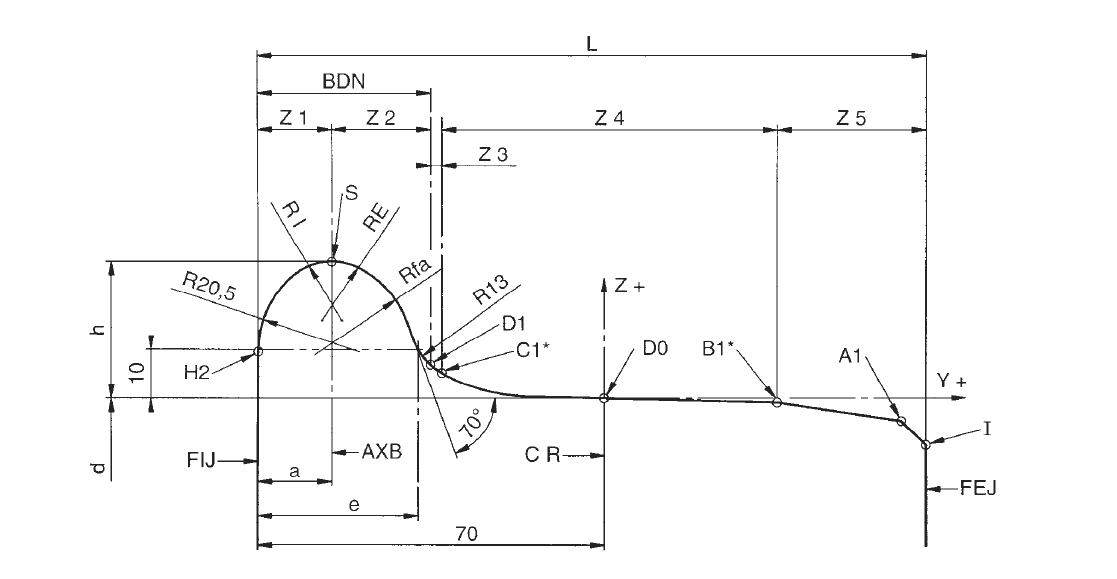
\includegraphics[width=\textwidth]{./images/wpms/uni_profile.png}
    \caption{Tread profile}
    \label{fig:uni-profile}
  \end{figure}

In the railway engineering is used to refer to wheels as \textit{wheelset}, that is a pair of wheels, fixed each other by an axle, obtaining a rotating solid (Figure \ref{fig:wheelset}). When a train is running, the two wheels belonging to the same wheelset rotate at the same speed: this is the reason why the flange is put in the inner side and the wheel is conical. During train's motion, it may happen that the wheelset is not perfectly centered with the rail, causing the wheel to hit the rail. In this case, the total motion of the wheelset is called ``winding motion''. Thanks to wheels geometry, this motion is damped gradually and rapidly, but the repeated hits wear out the profile of the wheel. The wider will be the oscillating motion, the stronger the damage to the wheel. \\
Another advantage of the conicity is when the train turns. In this case, centrifugal force pushes the wheelset to the outer side of the curve, allowing the inner wheel to rotate along a smaller diameter with respect to the outer wheel. Wheel measures reduce the number of crashing against the rail, which are, however, not null. Another way to decrease the number of these bumps is the rotation of the rails inwards. \\
All these effects greatly reduce safety during train travel, this is why an accurate and constant monitoring of the wheel status is fundamental. \\

Anyway, the great amount of detail makes the wheel reconstruction (from laser profile) a remarkably complex operation. To simplify the problem, some points of interest are usually identified (see Figures \ref{fig:uni-profile}, \ref{fig:keypoints} and \ref{fig:measures}), such as:  
  \begin{itemize}
    \item The rolling point $L_0$
    \item The flange top $S$
    \item The finishing point $H_0$ of the flange, on internal face of the wheel, and its symmetrical $Q_2$
    \item The finishing points of inner and outer faces
  \end{itemize}
Despite their simplicity, these points can provide all the measures reported in Table \ref{tab:measures}. In the same table will be also indicated some definition of interest, useful for our analysis. \\

  ~\\
  
  \begin{longtable}{|p{3cm}|c|p{8cm}|}
  \hline
  \multicolumn{1}{|c|}{\textbf{Element}}       & \textbf{Symbol} & \multicolumn{1}{c|}{\textbf{Definition}} \\
  \hline
  
  \textit{Active flange edge}                           &                 & Revolution surface comprised between two circumferences passing through the edge points $Q_1$ and $Q_2$. \\
  \hline
  \textit{Burr}                                         &                 & Metal outflow from the rolling surface to slide out. \\
  \hline
  \textit{External side of active flange edge}          & $Q_1$           & Point placed on the active face, at the radial distance of $2 mm$ from $S$ \\
  \hline
  \textit{Flange height}                                &  $h$            & Flange height, measured with respect to the tread.\\
  \hline
  \textit{Flange size}                                  & $S_d$           & Thickness measured at a radial distance of $10 mm$ from the tread.\\
  \hline
  \textit{Internal gauge}                               & $Si$            & Distance between the inner faces of the wheels of the same axle.\\
  \hline
  \textit{Internal side of the active flange edge}      & $Q_2$           & Point placed on the active face at the radial distance of $10 mm$ from the tread. \\
  \hline
  \textit{Nominal wheel diameter}                       &  $D$            & Design tread diameter. \\
  \hline
  \textit{Outboard gauge}                               & $Se$            & Distance between the active faces of the rims of the wheels of the same axle (reference points $Q_2$). \\
  \hline
  \textit{Qr quote}                                     & $Qr$            & Slope index of the active flange edge, i.e. the distance between the horizontal projections of the circumference passing from $Q_1$ and $Q_2$. \\
  \hline
  \textit{Thickness of the rim}                         & $Sc$            & Thickness measured at the rolling circle taking into account the surface roughness.\\
  \hline
  \textit{Tread}                                        &                 & Wheel circumference located at the intersection of an orthogonal plane to the wheel axis, at $70 mm$ distance from the inner face of the wheel. \\
  \hline
  \textit{Tread wear}                                   &                 & Crushing of the rolling surface, with material re-rolling towards the outer face. \\
  \hline
  \textit{Wheel diameter}                               &  $d$            & Tread diameter. \\
  \hline
  \textit{Width of rim}                                 &  $L$            & Distance between the vertical faces of the wheel rim or wheel crown. \\
  \hline
  
  \caption{Measures of interests and their definitions}
  \label{tab:measures}
\end{longtable}

  
  %\medskip
  \vfill
  
  \begin{figure}[h!]
    \centering
    \begin{minipage}[c]{.50\textwidth}
      \centering
      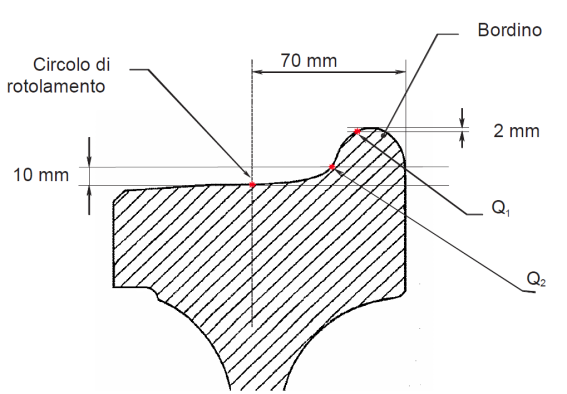
\includegraphics[width=0.95\textwidth]{./images/wpms/wheel-section.png}
        \caption{Wheel section keypoints}
    \label{fig:keypoints}
    \end{minipage}%
    \begin{minipage}[c]{.50\textwidth}
      \centering
      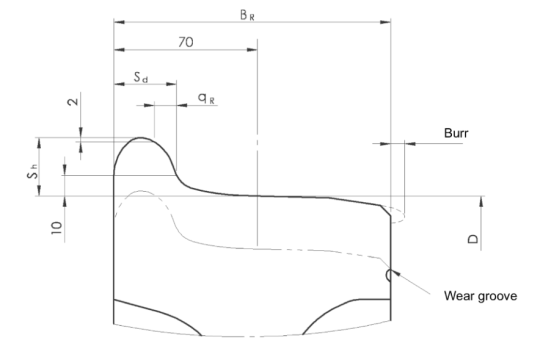
\includegraphics[width=1.05\textwidth]{./images/wpms/wheel_parameters.png}
      \caption{Wheel section measures}
      \label{fig:measures}
    \end{minipage}
  \end{figure}

  %\medskip
  \vfill

  \begin{figure}[h!]
    \centering
    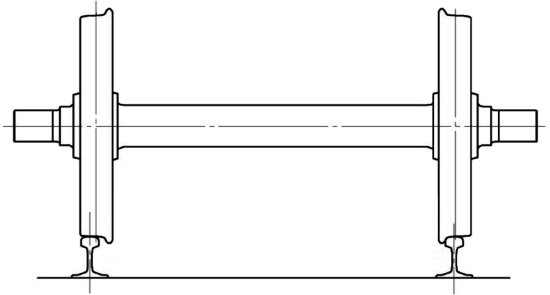
\includegraphics[width=0.7\textwidth]{./images/wpms/assile.jpg}
    \caption{Example of a wheelset}
    \label{fig:wheelset}
  \end{figure}

%  \begin{figure}[h!]
%    \centering
%    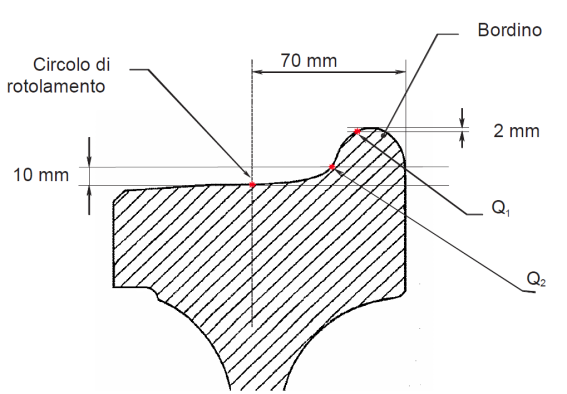
\includegraphics[width=0.6\textwidth]{./images/wpms/wheel-section.png}
%    \caption{Wheel section keypoints}
%    \label{fig:keypoints}
%  \end{figure}
%  \begin{figure}[h!]
%    \centering
%    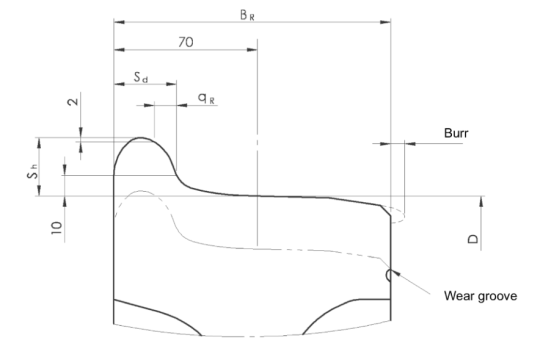
\includegraphics[width=0.6\textwidth]{./images/wpms/wheel_parameters.png}
%    \caption{Wheel section measures}
%    \label{fig:measures}
%  \end{figure}

% Needed to force next section to begin after figures
\clearpage

%%%%%%%%%%%%%%%%%%%%%%%%%%%

Wheel profile measurement system can be grouped into two categories, depending on the type of measurement, such as: \textit{static} measurement and \textit{dynamic} measurement.

In general, static measurement is performed in storage areas, during the maintenance of the train or of the wheel, when the train is stopped. This type of measures are done using mechanical calipers or optical methods: if we consider manual systems, the skill of the operator can influence seriously the results. Vice versa autonomous systems (typically based on optical sensors) are more precise and don't require any action of the operator. In both cases the main disadvantage is the fact that we have to disassemble the wheelset before performing the measures of interest, and as we said above, to achieve them periodically for each train is an impossible task.

Concerning dynamic systems, they allow to evaluate all the measures of interest while the train is running. These systems are typically based on contactless devices, such as electromagnetic or structured light sensors. Unlike mechanical sensors, these ones may also have a low resolution, but require a very good mathematical model that can process the collected data. In particular, structured light devices use at least two projector-camera pairs to avoid the problem of the occlusions. Furthermore, they need to collect at least three rolling points in different section of the profile to correctly evaluate the wheel diameter\cite{wpms-giuseppe}. Note that systems like these are more complex than the previous type: the high speeds of the trains and the serial acquisition of each axis need the presence of auxiliary technologies in order to detect the presence of a train, determine which axis is being analysed and pre-process collected data to reduce the transmission overhead. All this devices have to be synchronized if we want an high performance system. 
